\documentclass{standalone}
\usepackage{tikz}
\usepackage{color}
\usetikzlibrary{positioning, shapes, arrows.meta, calc, decorations.pathreplacing}

\definecolor{myblue}{RGB}{82,126,171}
\definecolor{myred}{RGB}{168, 50, 50}

\tikzset{
square/.style={draw,outer sep=5,inner sep=1,minimum size=10,line width=0, 
    very thick, draw=myblue, top color=white,bottom color=white}, 
  noborder/.style={draw,outer sep=0,inner sep=0,minimum size=20,line width=1, 
    draw=none, scale=1, anchor=west},
  blue/.style={draw,outer sep=35,inner sep=3,minimum size=20, line width=1, 
    very thick, draw=none, top color=myblue, bottom color=myblue, scale=1.25},
   noborderr/.style={draw,outer sep=0,inner sep=0,minimum size=20,line width=1, 
    draw=none, scale=1, anchor=west}
}

\begin{document}

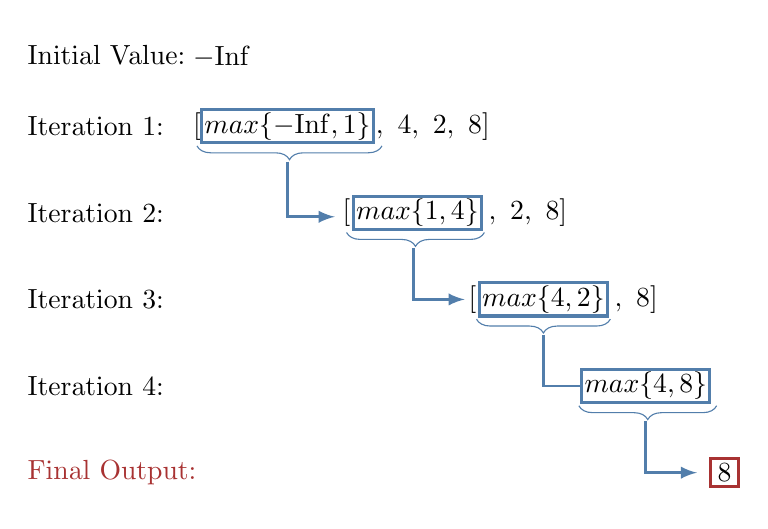
\begin{tikzpicture}


\draw[decorate,color=myblue,decoration={brace,amplitude=5pt}] (0.25,2.55) -- (-2.1,2.55);
\draw[-latex,line width=1 pt,color=myblue] (-0.95,2.35) |- (-0.35,1.65);


\node [noborderr] at (-2.15,3.68) {$-\mathrm{Inf}$};


%\node [noborderr] at (-2.25,2.8) {$[ 0+1, ~2, ~3,~ 4]$};
\node [noborderr] at (-2.15,2.8) {$[~~~~~~~~~~~~~~~~~~~, ~4, ~2, ~8]$};
\node [square] at (-0.95,2.8) {$max\{-\mathrm{Inf},1\}$};


\draw[decorate,color=myblue,decoration={brace,amplitude=5pt}] (1.55,1.45) -- (-0.2,1.45);
\draw[-latex,line width=1 pt,color=myblue] (0.65,1.25) |- (1.3,0.6);

\node [noborderr] at (-0.25,1.7) {$[~~~~~~~~~~~~~~~, ~2, ~8]$};
\node [square] at (0.7,1.7) {$max\{1,4\}$};


\draw[decorate,color=myblue,decoration={brace,amplitude=5pt}] (3.15,0.35) -- (1.45,0.35);
\draw[-latex,line width=1 pt, color=myblue] (2.3,0.15) |- (3,-0.5);

\node [noborderr] at (1.35,0.6) {$[~~~~~~~~~~~~~~~, ~8]$};
\node [square] at (2.3,0.6) {$max\{4,2\}$};


\draw[decorate,color=myblue,decoration={brace,amplitude=5pt}] (4.5,-0.75) -- (2.75,-0.75);
\draw[-latex,line width=1 pt,color=myblue] (3.6,-0.95) |- (4.25,-1.6);

\node [square] at (3.6,-0.5) {$max\{4,8\}$};
\node [square,draw=myred] at (4.6,-1.6) {$8$};


\node [noborderr] at (-4.25,3.7) {Initial Value:};
\node [noborderr] at (-4.25,2.8) {Iteration 1:};
\node [noborderr] at (-4.25,1.7) {Iteration 2:};
\node [noborderr] at (-4.25,0.6) {Iteration 3:};
\node [noborderr] at (-4.25,-0.5) {Iteration 4:};
\node [noborderr, color=myred] at (-4.25,-1.6) {Final Output:};



\end{tikzpicture}

\end{document}
